\documentclass{beamer}

\usetheme{Warsaw}

\setbeamertemplate{itemize items}[circle]


\usepackage[slovene]{babel}
\usepackage[utf8]{inputenc}
\usepackage[T1]{fontenc}
\usepackage{lmodern}

\usepackage{tikz}
\usetikzlibrary{calc, decorations.pathreplacing, positioning, arrows.meta, decorations.markings}

\usepackage{amsfonts, amsmath, amsthm}
\usepackage{enumitem}
\usepackage{graphicx}
\usepackage{import}


\usepackage{amssymb, mathrsfs}
\usepackage{color}
\usepackage{float}
\usepackage{booktabs}
\usetikzlibrary{calc, decorations.pathreplacing}
\usetikzlibrary{positioning, arrows.meta}
\usetikzlibrary{decorations.markings}

\tikzset{
    table_node/.style={inner sep=8pt},
    vnode/.style={circle, draw, fill=black, inner sep=0pt, minimum size=3pt},
    old_struct/.style={thin, black!40},
    old_edge/.style={thin, black!40},
    new_edge/.style={very thick, black},
    main_arrow/.style={-{Stealth}, line width=0.3pt, black},
    label_style/.style={font=\tiny, text=black!70},
    dashed_edge/.style={line width=1.0pt, black, dashed},
    old_edge_doily/.style={line width=1.1pt, black!70},
    v_point/.style={circle, draw=black, fill=white, inner sep=0pt, minimum size=5pt}
}
\newcommand{\tikznode}[2]{%
  \ifmmode
    \tikz[remember picture, baseline=(#1.base)]\node[inner sep=0pt, outer sep=0pt](#1){$#2$};%
  \else
    \tikz[remember picture, baseline=(#1.base)]\node[inner sep=0pt, outer sep=0pt](#1){#2};%
  \fi
}

% --- Teorematična okolja ---
\newtheorem{izrek}{Izrek}
\newtheorem{trditev}[izrek]{Trditev}
\newtheorem{posledica}[izrek]{Posledica}
\newtheorem{definicija}[izrek]{Definicija}
\newtheorem{zgled}[izrek]{Zgled}
\newtheorem{opomba}{Opomba}
\newtheorem{vprasanje}{Vprašanje}

% --- Ukazi ---
\newcommand{\red}{\operatorname{red}}
\newcommand{\srg}{\operatorname{srg}}
\newcommand{\diam}{\operatorname{diam}}
\newcommand{\N}{\mathbb{N}}
\newcommand{\ZZ}{\mathbb{Z}}
\newcommand{\reach}{\operatorname{Reach}}
\newcommand{\gr}{\mathscr{G}}
\newcommand{\aut}{\operatorname{Aut}}
\newcommand{\PG}{\operatorname{PG}}
\newcommand{\GF}{\operatorname{GF}}

\newcommand{\A}{\mathcal{A}}
\newcommand{\II}{\mathbf{I}}
\newcommand{\IIw}[2]{#1 \;\II\; #2}
\newcommand{\IIwd}[2]{#1 \;\II^D\; #2}
\newcommand{\PP}{\mathcal{P}}
\newcommand{\LL}{\mathcal{L}}

\newcommand{\fig}[2]{%
  \begin{figure}
    \centering
    \resizebox{#1}{!}{\import{../../assets/}{#2}}
  \end{figure}
}
\newcommand{\figH}[2]{%
  \begin{figure}
    \centering
    \resizebox{!}{#1}{\import{../../assets/}{#2}}
  \end{figure}
}


% --- Naslov ---
\title{Mooreovi grafi in posplošeni večkotniki}
\author{Luka Lavš}
\date{28. avgust 2026}

\begin{document}

% --- Title ---
\begin{frame}
    \titlepage
\end{frame}

% ------------------------------
\section{Mooreovi grafi}

\begin{frame}
    \frametitle{Premer in ožina grafa}
    \begin{definicija}
        \textbf{Premer} grafa je največja razdalja med njegovima vozliščema, 
        \textbf{ožina} pa je dolžina
        njegovega najkrajšega cikla.
    \end{definicija}
    \fig{0.42\textwidth}{grid-caterpilar.tex}
    \begin{center}
        \small $4\times 4$ mreža ima premer $6$ in ožino $4$, medtem ko ima drevo 
        na sliki premer $5$ in neskončno ožino.
    \end{center}
\end{frame}

\begin{frame}
    \frametitle{Mooreovi grafi}
    \begin{vprasanje}
        Kako velik je lahko graf z maksimalno stopnjo $\Delta$ in 
        premerom kvečjemu $D$?
    \end{vprasanje}
    \begin{definicija}
        \emph{Mooreovi grafi} so tisti, ki za dan premer $D$ in maksimalno stopnjo $\Delta$
        dosegajo zgornjo mejo števila vozlišč
        \[M^{\Delta, D} = 1 + \Delta + \Delta (\Delta - 1) + \ldots + \Delta (\Delta - 1)^{D-1},\]
        ki ji pravimo \emph{Mooreova meja}.
    \end{definicija}
\end{frame}

\begin{frame}
    \begin{definicija}
        \emph{Mooreovo drevo} $T_{\Delta, D}$ je drevo z globino $D$, kjer ima koren
        stopnjo $\Delta$, vsa ostala notranja vozliča pa stopnjo $\Delta - 1$.
    \end{definicija}
    \fig{0.42\textwidth}{drevo-moore-uvod.tex}
    \begin{center}
        \small Mooreovo drevo $T_{7, 2}$ ima $1 + 7 + 7\cdot 6 = 50$ vozlišč.
    \end{center}

    \begin{trditev}
        Graf premera $D$ in max.~stopnje $\Delta$ je Mooreov natanko tedaj, ko je njegova ožina $g$ enaka $2D+1$, oz.~%
        ko je vsako vozlišče v grafu koren
        nekega podgrafa, ki je izomorfen Mooreovemu drevesu $T_{\Delta, D}$.
    \end{trditev}
\end{frame}

\begin{frame}
    \frametitle{Trivialni Mooreovi grafi}
    \begin{trditev}
        Lihi cikli $C_{2D+1}$ so Mooreovi grafi za poljuben premer $D$ in stopnjo $2$,
        medtem ko so polni grafi $K_{\Delta+1}$ Mooreovi grafi za poljubno stopnjo $\Delta$ in premer $1$.
    \end{trditev}
    \begin{center}
    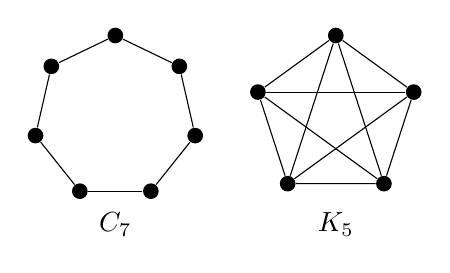
\begin{tikzpicture}[scale=0.8, vnode/.style={circle, fill=black, inner sep=2pt}]
        % C_7
        \foreach \i in {1,...,7}
            \node[vnode] (c\i) at ({90-360*(\i-1)/7}:1.3) {};
        \foreach \i in {1,...,7} {
            \pgfmathtruncatemacro{\nexti}{mod(\i,7)+1}
            \draw (c\i) -- (c\nexti);
        }
        \node at (0,-1.7) {$C_7$};
        % K_5
        \begin{scope}[xshift=3.5cm]
        \foreach \i in {1,...,5}
            \node[vnode] (k\i) at ({90-360*(\i-1)/5}:1.3) {};
        \foreach \i in {1,...,5} {
            \foreach \j in {\i,...,5} {
                \ifnum\i<\j
                    \draw (k\i) -- (k\j);
                \fi
            }
        }
        \node at (0,-1.7) {$K_5$};
        \end{scope}
    \end{tikzpicture}
    \end{center}
\end{frame}

\begin{frame}
    \frametitle{Lastnosti Mooreovih grafov}
    \begin{definicija}
        Graf je \emph{razdaljno regularen} natanko tedaj, ko je regularen in je število vozlišč, ki so 
        na razdalji $j$ od vozlišča $u$ in $k$ od vozlišča $v$ odvisno le od razdalje 
        med $u$ in $v$, $j$ in $k$.
    \end{definicija}
    \begin{trditev}
        Mooreovi grafi so razdaljno regularni.
    \end{trditev}

    \begin{definicija}
        Graf je krepko regularen natanko tedaj, ko je regularen in imata vsaki dve sosednji vozlišči
        natanko $\lambda$ skupnih sosedov, vsaki dve nesosednji vozlišči pa natanko $\mu$ skupnih sosedov.
    \end{definicija}
    \begin{trditev}
        Mooreovi grafi premera $2$ so krepko regularni z $\lambda = 0$ in $\mu = 1$.
    \end{trditev}
\end{frame}


\begin{frame}
    \frametitle{Obstoj Mooreovih grafov}
    \begin{trditev}
        Če je $A$ matrika sosednosti Mooreovega grafa premera $D$ in stopnje
        $\Delta$, potem velja Mooreova matrična enačba
        \[
            G^{\Delta,D}(A)=J,
        \]
        kjer je $J$ matrika samih enic.
    \end{trditev}
    \vspace{0.3cm}
    \begin{trditev}
        Za premer $D=2$ se ta enačba poenostavi v
        \[
            \boxed{A^2+A-(\Delta-1)I=J.}
        \]
    \end{trditev}
\end{frame}

\begin{frame}
    \begin{izrek}
    Mooreovi grafi s premerom $D\geq 3$, z izjemo lihih ciklov $C_{2D+1}$, ne obstajajo.
    \end{izrek}
    \begin{izrek}
        Mooreovi grafi s premerom $D=2$ obstajajo zgolj morda 
        za stopnje $\Delta \in \{2, 3, 7, 57\}$.
    \end{izrek}
    \begin{trditev}
        Mooreov graf s premerom $D=2$ in stopnjo $\Delta = 3$ je Petersenov graf.
        \fig{0.7\textwidth}{petersen-drevo.tex}
    \end{trditev}
\end{frame}

\begin{frame}
    \frametitle{Hoffman-Singletonov graf}
    \begin{trditev}
        Mooreov graf s premerom $D=2$ in stopnjo $\Delta = 7$ imenujemo Hoffman-Singletonov graf.
        Sestavljen je iz petih petkotnikov $Q_0, \ldots, Q_4$ ter petih komplementarnih zvezd 
        $P_0, \ldots, P_4$, ki so med seboj povezani s pravilom:
        \begin{align*}
            Q_i^a \sim P_j^{a + ij \bmod{5}} &&\text{in}&& P_j^b \sim Q_i^{b - ij \bmod{5}}
        \end{align*}
        \begin{center}
            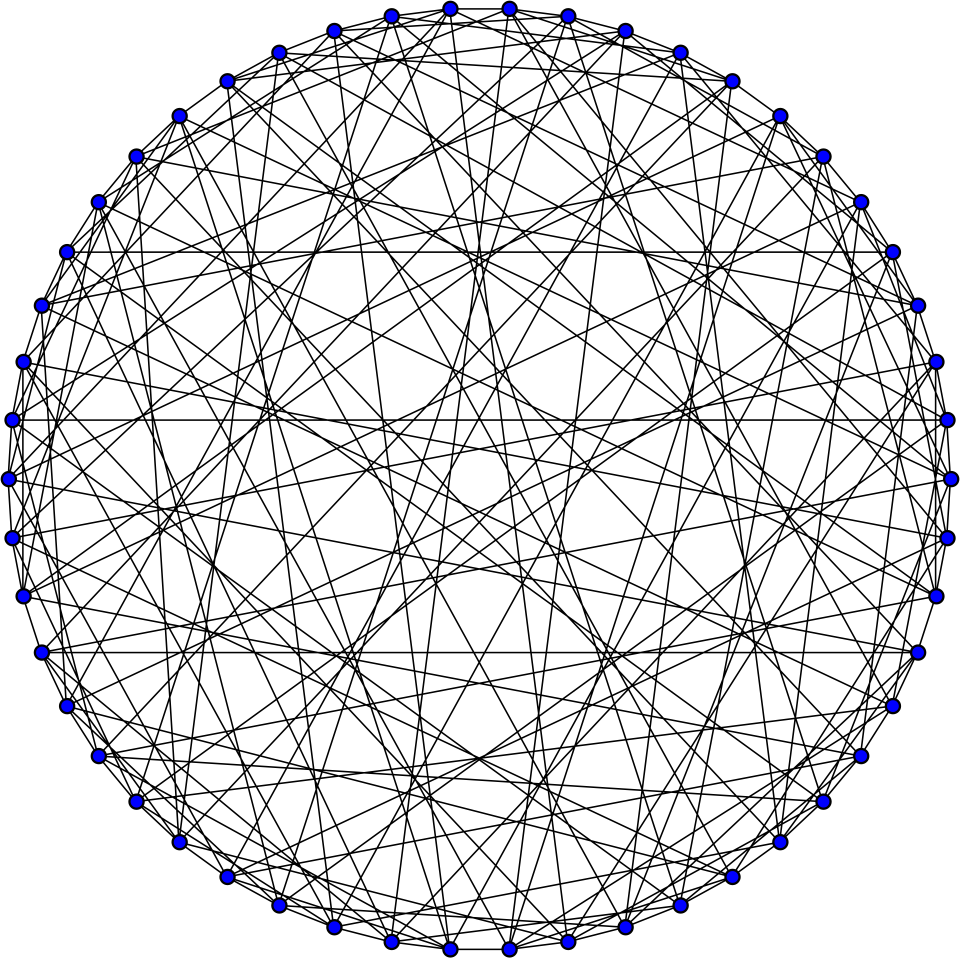
\includegraphics[width=0.3\textwidth]{../../assets/hoffman-singelton-graph.png}
        \end{center}
    \end{trditev}
\end{frame}

\begin{frame}
    \frametitle{Aschbacherjev graf}
    \begin{trditev}
        Mooreov graf s premerom $D=2$ in stopnjo $\Delta = 57$ je še vedno neznan, vendar je znano, 
        da če obstaja, ni vozliščno tranzitiven. Še več, red njegove grupe avtomorfizmov,
        ki ne vsebuje niti involucij, je 
        navzgor omejen s $375$.
    \end{trditev}
    \begin{trditev}
        Aschbacherjev graf ima $3250$ vozlišč. Njegov spekter pa je enak
        \[\{57^{(1)}, 7^{(1729)}, (-8)^{(1520)}\}.\]
    \end{trditev}
    \begin{opomba}
        Pri njegovi analizi se običajno opazuje predvsem podgrafe $\operatorname{Fix}(\tau)$,
        ki so inducirani z vozlišči, ki jih fiksira izbran avtomorfizem $\tau$.
    \end{opomba}
\end{frame}

\begin{frame}
    \frametitle{Mooreova meja kot spodnja meja}
    \begin{trditev}
        Spodnja meja za število vozlišč v grafu z ožino $g$ in minimalno stopnjo $\Delta$ znaša
        \[M^{\Delta, \frac{g - 1}{2}}.\]
    \end{trditev}
    \begin{opomba}
        Spodnjo mejo je mogoče izboljšati za primer dvodelnih grafov, kjer je ožina soda.
        Grafom, ki tako mejo dosežejo, pravimo \emph{dvodelni Mooreovi grafi}.
    \end{opomba}
    \fig{0.35\textwidth}{dvodelno-mooreovo-drevo.tex}
    \begin{center}
        \small Dvodelno Mooreovo drevo $T^{[2]}_{\Delta, D}$ ima\\
        $2 + 2(\Delta - 1) + \ldots + 2(\Delta - 1)^{D-1}$ vozlišč.
    \end{center}
\end{frame}


\begin{frame}
    \frametitle{Dvodelni Mooreovi grafi}
    \begin{trditev}
        Graf je dvodelni Mooreov graf natanko tedaj, ko je regularen s premerom $D$ in ožino $g=2D$,
        oz.~ko sta poljubni dve vozlišči vsebovani v nekem $C_{2D}$ ter v grafu ni ciklov 
        krajših od $2D$.
    \end{trditev}
    \begin{opomba}
        Ker so dvodelni Mooreovi grafi dvodelni, lahko njihova vozlišča razdelimo v dve množici 
        $\PP$ in $\LL$, kjer vozliščem množice $\PP$ pravimo \emph{točke}, 
        vozliščem množice $\LL$ pa \emph{premice}.
    \end{opomba}
    \fig{0.6\textwidth}{prehod-v-geometrijo-trikotnik.tex}
    \begin{center}
        \small Uvedemo pojem običajnega večkotnika.
    \end{center}
\end{frame}

\begin{frame}
    \frametitle{Posplošeni večkotniki}
    \begin{definicija}
        Geometrijsko interpretacijo grafa formalno zapišemo kot geometrijo $\Gamma = (\PP, \LL, \II)$ 
        ranga $2$, kjer je $\PP$ množica točk, $\LL$ množica premic, $\II$ pa relacija incidence.
    \end{definicija}
    \begin{definicija}
        \emph{Posplošeni $n$-kotnik} je geometrija ranga $2$, kjer poljubna dva 
        elementa $x, y\in \PP\cup\LL$ ležita v nekem običajnem $n$-kotniku, in kjer ni običajnih
        $m$-kotnikov za $m < n$.
    \end{definicija}
    \begin{definicija}
        Dvodelni Mooreovi grafi so natanko regularni posplošeni $n$-kotniki, kjer je $n = \frac{g}{2} = D$.
    \end{definicija}
\end{frame}

\begin{frame}
    \frametitle{Regularni posplošeni večkotniki}
    \begin{izrek}
        $\Delta$-regularni posplošeni $D$-kotniki obstajajo le za $\Delta = 2$ in so običajni 
        $D$-kotniki, ali pa za $D\in\{2, 3, 4, 6\}$.
    \end{izrek}
    \begin{opomba}
        Običajni $D$-kotniki so ravno sodi cikli $C_{2D}$, medtem ko so 
        posplošeni $2$-kotniki ravno polni dvodelni grafi $K_{\Delta, \Delta}$.
        \fig{0.75\textwidth}{dvokotnik.tex}
    \end{opomba}
\end{frame}


\begin{frame}
    \frametitle{Projektivne ravnine}
    \begin{definicija}
        Projektivne ravnine so regularni posplošeni $3$-kotniki, izključujoč običajne $3$-kotnike. 
        Alternativno so definirane z naslednjimi aksiomi:
        \begin{enumerate}[label=(\roman*), noitemsep, topsep=1pt]
            \footnotesize
            \item Vsaki dve točki povezuje natanko ena premica.
            \item Vsaki dve premici se sekata v natanko eni točki.
            \item Obstajajo take štiri točke, da nobena premica ne nosi več\\ kot dveh izmed njih.
        \end{enumerate}
    \end{definicija}
    \begin{opomba}
        V končnem vektorskem prostoru $\mathbb{K}^3$ vsaki dve premici določata natanko 
        eno ravnino in vsaki dve ravnini določata natanko eno premico. S tem ko 
        za množico točk $\PP$ vzamemo vse premice v $\mathbb{K}^3$, za množico premic 
        $\LL$ pa vse ravnine v $\mathbb{K}^3$, ob incidenci vsebovanosti dobimo projektivno ravnino
        -- natančneje Desarguesovo ravnino $\PG(2, \mathbb{K})$.
    \end{opomba}
\end{frame}

\begin{frame}
    \fig{0.75\textwidth}{fano-pg2.tex}
    \begin{center}
        \small Najmanjša projektivna ravnina je Fanova ravnina $\PG(2, \GF(2))$, 
        ki ima $7$ točk in $7$ premic.
    \end{center}
    \begin{opomba}
        Obstajajo tudi ne-Desarguesove projektivne ravnine, ki jih ni mogoče dobiti iz 
        vektorskih prostorov. Njihovo konstrukcijo je mogoče opisati z
        \emph{ravninskimi tričlenimi kolobarji} $(\mathbb{T}, T)$, kjer je $\mathbb{T}$ 
        množica točk, $T: \mathbb{T}^3 \to \mathbb{T}$ pa preslikava, ki zadošča določenim
        aksiomom. 
    \end{opomba}
\end{frame}

\begin{frame}
    \frametitle{Regularni posplošeni $4$-kotniki}
    \begin{definicija}
        Simplektični posplošeni $4$-kotnik $W(\mathbb{K})$ je geometrija ranga $2$, 
        kjer so točke vse točke iz $\PG(3, \mathbb{K})$, 
        premice pa vse premice iz $\PG(3, \mathbb{K})$, za katere velja 
        $L^\tau = L$ za simplektično polarnost $\tau$ s predpisom
        \[L^\tau = \{x\in \mathbb{K}^4 \mid \forall y\in L:\, \langle x, y\rangle = 0\},\]
        kjer je $\langle x, y\rangle = x_1y_2 - x_2y_1 + x_3y_4 - x_4y_3$.
    \end{definicija}
    \begin{definicija}
        Premici $L \in PG(d, \mathbb{K})$, ki jo določata dve različni točki s 
        homogenimi koordinatami $(x_0, \ldots, x_d)$ in $(y_0, \ldots, y_d)$, pripadajo \emph{Grassmanove koordinate}
       $p_{ij} =
            \begin{vmatrix}
                x_i & x_j \\
                y_i & y_j
            \end{vmatrix}
        $
        za vse $0 \le i < j \le d$. Premice iz $\PG(d, \mathbb{K})$ lahko tako predstavimo 
        kot točke v $\PG(\binom{d+1}{2} - 1, \mathbb{K})$.
    \end{definicija}
\end{frame}

\begin{frame}
\fig{0.75\textwidth}{doly-accurate.tex}
\begin{center}
    \small Najmanjši simplektični posplošeni $4$-kotnik ima $15$ točk in $15$ premic. 
\end{center}
\end{frame}


\begin{frame}
    \begin{definicija}
        Ortogonalni posplošeni $4$-kotnik $Q(4, \mathbb{K})$ je geometrija ranga $2$
        z incidenco vsebovanosti,
        kjer so točke vsi $1$-dimenzionalni podprostori iz $q^{-1}(0)$, premice pa vsi 
        $2$-dimenzionalni podprostori iz $q^{-1}(0)$, za parabolično kvadratno 
        formo $q(x_0, \ldots, x_4) = x_0x_1 + x_2x_3 + x_4^2$ v prostoru $\mathbb{K}^5$ oz. 
        v $\PG(4, \mathbb{K})$.
    \end{definicija}
    \fig{0.38\textwidth}{doily-incidence.tex}
    \begin{center}
        \small Najmanjši ortogonalni posplošeni $4$-kotnik, prikazan kot graf.
    \end{center}
\end{frame}

\begin{frame}
    \begin{trditev}
        Simplektični in ortogonalni posplošeni $4$-kotnik sta si dualna. To pomeni,
        da se zgolj zamenjata vlogi točk in premic, pri čemer ostane relacija 
        incidence nespremenjena.
    \end{trditev}
    \begin{trditev}
        Edina druga znana družina regularnih posplošenih $4$-kotnikov je družina 
        \emph{Titsovih posplošenih $4$-kotnikov} $T_2(\mathcal{O})$.
    \end{trditev}
\end{frame}


\begin{frame}
    \frametitle{Posplošeni $6$-kotniki}
    \begin{opomba}
        Edini znani regularni posplošeni $6$-kotniki so \emph{razdeljeni Cayleyjevi 
        posplošeni $6$-kotniki} $H(\mathbb{{K}})$, ki jih je mogoče konstruirati na način,
        soroden konstrukciji ortogonalnih posplošenih $4$-kotnikov.
    \end{opomba}
    \fig{0.25\textwidth}{generalized-hexagon-h2.tex}
    \begin{center}
        \small Najmanjši razdeljeni Cayleyjev posplošeni $6$-kotnik\\ ima $63$ točk in $63$ premic.
    \end{center}
\end{frame}

\begin{frame}
    \frametitle{Sorodne teme}
    \begin{opomba}
        Vprašanje obstoja Aschbacherjevega grafa in popolne klasifikacije 
        regularnih posplošenih večkotnikov ostaja odprto.
    \end{opomba}
    \begin{opomba}
        Sorodna področja so \emph{Mooreovi grafi z defektom}, 
        \emph{teorija kletk} in \emph{teorija zgradb}, ki se ukvarjajo z grafi 
        blizu Mooreove meje, grafi z minimalnim številom vozlišč ter strukturnimi 
        lastnostmi regularnih posplošenih večkotnikov.
    \end{opomba}
\end{frame}

\begin{frame}
    \fig{0.25\textwidth}{defect-2.tex}
    \begin{center}
        \small $3$-regularen graf s premerom $2$ in defektom $-2$.
    \end{center}
    \fig{0.25\textwidth}{mcgee-cage.tex}
    \begin{center}
        \small $3$-regularen graf s premerom $4$ in ožino $7$, ki je kletka.
    \end{center}
\end{frame}



\end{document}
